\documentclass[12pt,a4paper]{amsart}
\usepackage[UTF8]{ctex}
\usepackage{preamble}

% 定义 example 环境
\newcounter{example}[section] % 定义 example 计数器
\newenvironment{example}{%
    \refstepcounter{example}% 增加计数器
    \par\medskip\noindent
    \textbf{Example \theexample:}\ %
}{%
    \par\medskip
}

% 定义 solution 环境
\newcounter{solution}[section] % 定义 solution 计数器
\newenvironment{solution}{%
    \refstepcounter{solution}% 增加计数器
    \par\medskip\noindent
    \textbf{Solution \thesolution:}\ %
}{%
    \par\medskip
}

\title{Chapter 2 随机变量}

\begin{document}

\maketitle\cite{杨振明2007}

\section{随机变量}

\begin{definition}[随机变量]
    设 $(\Omega, \mathcal{F}, P)$ 为概率空间,$\xi = \xi(\omega): \Omega\to\R$,若
    \begin{equation}
        \{\omega: \xi(\omega) < x\} \in \mathcal{F}, \quad \forall x \in \R
    \end{equation}
    则称 $\xi$ 为随机变量
\end{definition}

注:$\xi(\omega)$ 可简写为 $\xi$,$\xi(\omega) < x$ 可简写为 $\xi < x$

随机变量的逆变换有如下性质

\begin{proposition}
    设 $\xi$ 为随机变量,其逆变换为 $\xi^{-1}$,则
    \begin{enumerate}
        \item $\xi^{-1}(\R)=\Omega$
        \item $\forall B\subseteq C \Rightarrow \xi^{-1}(B) \subseteq \xi^{-1}(C)$
        \item $\xi^{-1}(\overline{B}) = \overline{\xi^{-1}(B)}$
        \item $\xi$ 的 Borel 函数仍为随机变量
    \end{enumerate}
\end{proposition}

\begin{proposition}[随机变量的结构]
    \begin{enumerate}
        \item $(\Omega, \mathcal{F}, P)$ 中 $E\in F$ 的示性函数 $\mathbb{1}_E(\omega)$ 为随机变量
        \item 设 $(\Omega, \mathcal{F}, P)$ 为 R.V. $\Leftrightarrow$ $\exists$ 简单随机变量列 $\{\xi_n\}_{n\geq 1}$ $s.t. \lim\limits_{n\to\infty}\xi_n(\omega)=\xi(\omega), \forall\omega\in\Omega$(此处极限为逐点收敛)
    \end{enumerate}
\end{proposition}

\section{随机分布(分布)}

\begin{definition}[分布]
    $(\Omega, \mathcal{F}, P)$ 为概率空间,$\mathbb{F}(B) = P\{\xi^{-1}(B)\} = P\{\xi\in B\}, \forall B\in\mathcal{B}$,则 $\mathbb{F}$ 为一个概率测度,称作 $\xi$ 的概率分布
\end{definition}

$\mathbb{F}$ 刻画了 $\xi$ 的分布规律

\begin{definition}[相空间]
    $(\R, \mathcal{B}, \mathbb{F})$ 为 $\xi$ 的相空间,$\mathbb{F}$ 与 $\xi$ 有关
\end{definition}

\begin{definition}[分布函数]
    $F(x) = \mathbb{F}((-\infty, x]) = P\{\xi\leq x\}, \forall x\in\R$,称 $F(x)$ 为 $\xi$ 的分布函数
\end{definition}

分布函数具有以下性质

\begin{proposition}
    \begin{enumerate}
        \item $F(x)$ 单调不减,即 $x_1\leq x_2 \Rightarrow F(x_1)\leq F(x_2)$   
        \item $F(x)$ 左连续,即 $x_0\in\R \Rightarrow \lim\limits_{x\to x_0^-}F(x)=F(x_0)$
        \item $F(-\infty) = \lim\limits_{x\to-\infty}F(x)=0, F(+\infty) = \lim\limits_{x\to+\infty}F(x)=1$
    \end{enumerate}
\end{proposition}

\begin{definition}[离散型]
    $(\Omega, \mathcal{F}, P)$ 为概率空间,$\xi$ 为随机变量,若 $\exists \{x_k\}, \{p_k\}$ 使得
    \begin{equation}
        p_k \geq 0, \sum_{k}p_k = 1, P\{\xi = x_k\} = p_k, \forall k
    \end{equation}
    则称 $\xi$ 为离散型随机变量,其密度阵
    \begin{equation}
        \begin{pmatrix}
            x_1 & x_2 & \cdots & x_n \\
            p_1 & p_2 & \cdots & p_n
        \end{pmatrix}
    \end{equation}
\end{definition}

\begin{definition}[连续型]
    $(\Omega, \mathcal{F}, P)$ 为概率空间,$\xi$ 为随机变量,若 $\exists p(x)$ 使得
    \begin{equation}
        p(x) \geq 0, \int_{-\infty}^{+\infty}p(x)dx = 1, P\{\xi=a\} = 0, \forall a
    \end{equation}
    则称 $\xi$ 为连续型随机变量,其密度函数为 $p(x)$
\end{definition}

不管是什么类型的随机变量,我们都有

\begin{proposition}[Lebesgue 分解]
    任意分布函数 $F(x)$ 可分解为
    \begin{equation}
        F(x) = c_1F_1(x) + c_2F_2(x) + c_3F_3(x)
    \end{equation}
    其中 $F_1(x)$ 为纯条约分布函数,$F_2(x)$ 为连续型分布函数,$F_3(x)$ 为奇异分布函数
\end{proposition}

\section{一些典型分布}

\subsection{二项分布}

$\xi\sim B(n,p)$

\begin{definition}[二项分布]
    设 $n$ 次独立重复试验,每次试验成功的概率为 $p$,失败的概率为 $1-p$,则 $\xi$ 为成功次数,$\xi\sim B(n,p)$
\end{definition}

\begin{proposition}[二项分布的分布函数]
    \begin{equation}
        P\{\xi=k\} = \binom{n}{k}p^k(1-p)^{n-k}
    \end{equation}
\end{proposition}

\subsection{几何分布}

$\xi\sim G(p)$

\begin{definition}[几何分布]
    设独立重复试验,每次试验成功的概率为 $p$,失败的概率为 $1-p$,则 $\xi$ 为第一次成功所需的试验次数,$\xi\sim G(p)$
\end{definition}

\begin{proposition}[几何分布的分布函数]
    \begin{equation}
        P\{\xi=k\} = (1-p)^{k-1}p
    \end{equation}
\end{proposition}

\subsection{Pascal 分布(负二项分布)}

$\xi\sim F(n,p)$

\begin{definition}[Pascal 分布]
    设独立重复试验,每次试验成功的概率为 $p$,失败的概率为 $1-p$,则 $\xi$ 为第 $n$ 次成功所需的试验次数,$\xi\sim F(n,p)$
\end{definition}

\begin{proposition}[Pascal 分布的分布函数]
    \begin{equation}
        P\{\xi=k\} = \binom{k-1}{n-1}p^n(1-p)^{k-n}
    \end{equation}
\end{proposition}

\subsection{Poisson 分布}

$\xi\sim P(\lambda)$

\begin{definition}[Poisson 分布]
    设独立重复试验,每次试验成功的概率为 $\lambda/n$,失败的概率为 $1-\lambda/n$,则 $\xi$ 为成功次数,$\xi\sim P(\lambda)$
\end{definition}

\begin{proposition}[Poisson 分布的分布函数]
    \begin{equation}
        P\{\xi=k\} = \frac{\lambda^k}{k!}e^{-\lambda}
    \end{equation}
\end{proposition}

\subsection{正态分布}

$\xi\sim N(\mu, \sigma^2)$

\begin{definition}[正态分布]
    设 $\xi$ 服从正态分布 $N(\mu, \sigma^2)$,则其密度函数为
    \begin{equation}
        p(\xi) = \phi_{\mu,\sigma} (\xi) = \frac{1}{\sqrt{2\pi}\sigma}e^{-\frac{(\xi-\mu)^2}{2\sigma^2}}
    \end{equation}
\end{definition}

\begin{proposition}[正态分布的分布函数]
    \begin{equation}
        F(x) = \frac{1}{\sqrt{2\pi}\sigma}\int_{-\infty}^{x}e^{-\frac{(t-\mu)^2}{2\sigma^2}}dt
    \end{equation}
\end{proposition}

\subsection{Gamma 分布}

$\xi\sim \Gamma(\lambda, r)$

\begin{definition}[Gamma 分布]
    设 $\xi$ 服从 Gamma 分布 $\Gamma(\lambda, r)$,其中 $\lambda>0, r>0$,则其密度函数为
    \begin{equation}
        p(\xi) = \frac{\lambda^r}{\Gamma(r)}\xi^{r-1}e^{-\lambda\xi}
    \end{equation}
\end{definition}

\begin{proposition}[Gamma 分布的分布函数]
    \begin{equation}
        F(x) = \frac{\lambda^r}{\Gamma(r)}\int_{0}^{x}t^{r-1}e^{-\lambda t}dt
    \end{equation}
\end{proposition}

\subsection{指数分布}

Gamma 分布中 $r=1$ 的情形,$\xi\sim E(\lambda)$

\begin{definition}[指数分布]
    设 $\xi$ 服从指数分布 $E(\lambda)$,则其密度函数为
    \begin{equation}
        p(\xi) = \lambda e^{-\lambda\xi}
    \end{equation}
\end{definition}

\begin{proposition}[指数分布的分布函数]
    \begin{equation}
        F(x) = \int_{0}^{x}\lambda e^{-\lambda t}dt
    \end{equation}
\end{proposition}

\subsection{各种分布的关系}

\begin{figure}[htbp]
    \centering
    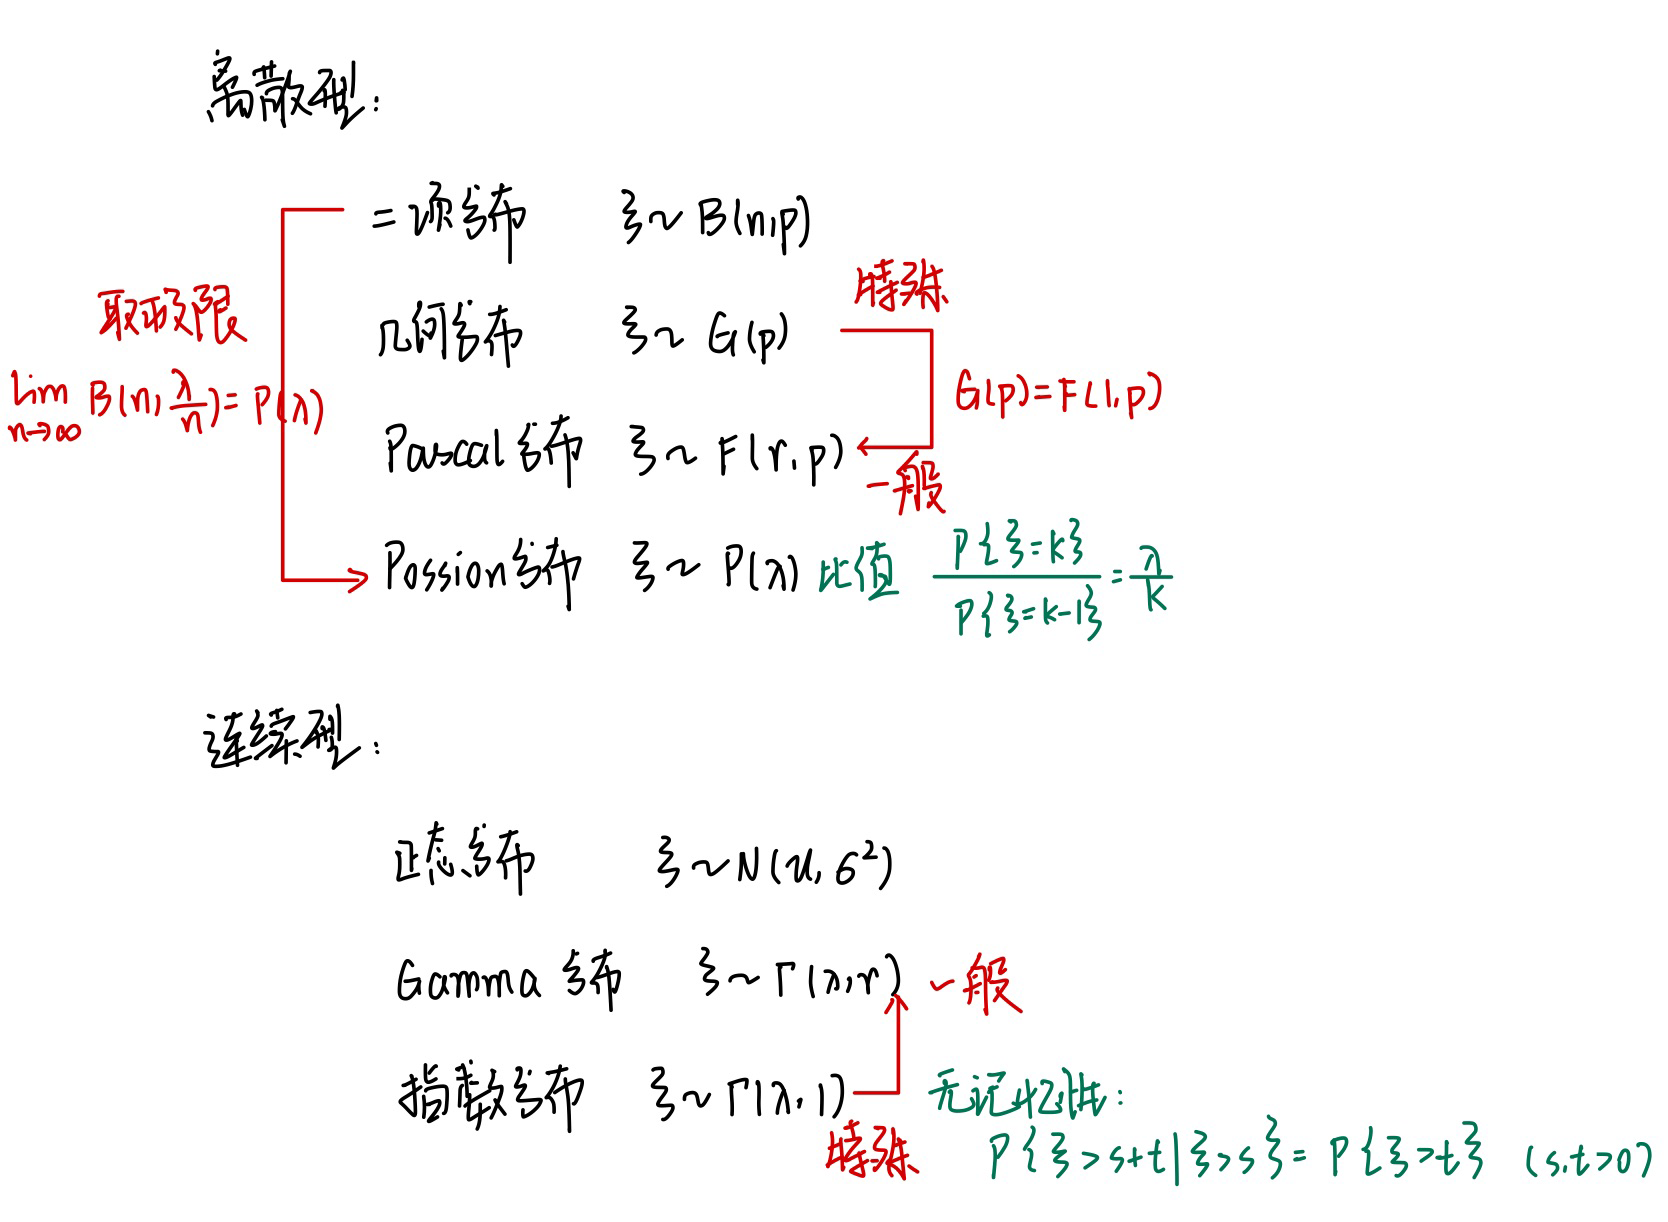
\includegraphics[width=0.8\textwidth]{./src/1.png}
    \caption{各种分布的关系}
    \label{fig:1}
\end{figure}

\section{多维概率分布}

\appendix


\bibliographystyle{unsrt}
{\footnotesize\bibliography{./library}}


\end{document}
